% Chapter Template
\chapter{Related Work} % Main chapter title

\label{Chapter 2} % Change X to a consecutive number; for referencing this
% chapter elsewhere, use \ref{ChapterX}

\lhead{Chapter 2. \emph{Related Work}} % Change X to a consecutive number; this
% is for the header on each page - perhaps a shortened title

\begin{table}[ht]
\centering
\begin{tabular}{| c | c | c | c | c | c |}
\hline
Tool & Layers & Dia.   & Const. & Platform & GUI\\
	 & 		  & Const. & Language & & \\
\hline
EMF/GMF & 2 & & OCL, EVL, & Java VM & $\surd$ \\
\hline
VMTS & \infty & & OCL, EVL, & Java VM & $\surd$ \\
\hline
AToM & 2 & & OCL, EVL, & Java VM & $\surd$ \\
\hline
GME & 2 & & OCL, EVL, & Java VM & $\surd$ \\
\hline
metaDepth & \infty & & OCL, EVL, & Java VM & \\
\hline
DPF & \infty & & OCL, EVL, & Java VM & $\surd$ \\
\hline

\end{tabular}
\caption{Comparing model transformation tools.}
\end{table}

%----------------------------------------------------------------------------------------
%	SECTION 1
%----------------------------------------------------------------------------------------

\section{Graph Transformation}
\noindent One approach to model transformations is by graph transformations,
also referred to as graph rewriting. Graph rewriting can be implemented with
an algebraic approach, which is based upon category theory\cite{Barr1990}.

\begin{figure}[htbp]
  \centering
    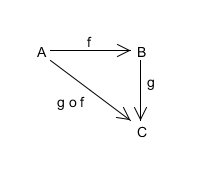
\includegraphics{./Figures/categoryTheory.png}
    \rule{35em}{0.5pt}
  \caption[Collection of objects for category theroy graph]{Collection of
  objects A,B and C.}
  \label{fig:categoryTheory}
\end{figure}


In category theory there are a collection of objects and arrows. These arrows
are also called morphisms. In figure~\ref{fig:categoryTheory} we have a
collection of objects A, B and C and morphisms f, g and g $\circ$ f. And for the
purpose of this paper, the collection of objects are graphs and the arrows are
graph morphisms. This is also very typical when writing papers to explain the
concepts of graph transformations, where these objects are represented as
graphs, and arrows are represented as morphisms. Category theory can then be
used to formalize the concepts at a high level of abstraction.

\subsection{The Algebraic Approach}
\noindent This approach are based on the concepts of composing graphs, modelled
by pushouts of graphs and graph morphisms. This pushout approach comes in
different categories, and we will look at two of these, namely the
double-pushout (DPO) approach and the single pushout (SPO) approach\cite{Loewe1997,Ehrig1997}.

\indent Historically, the first of the algebraic approaches to graph
transformations, the double-pushout, was first introduced at the Technical
University of Berlin in the early seventies by H. Ehrig, M. Pfender and H.J.
Schneider\cite{INSPEC:606170}. They tried to generalize Chromsky grammars from
strings to graphs. This allowed to define a graph rewriting step by the use of
two gluing constructions. And by applying a graph rewriting step for the
double-pushout approach is a pair of morphisms in the category of graphs where
the arrows represents total graph morphisms, \linebreak\mbox{L $\longleftarrow$
\ K $\longrightarrow$ R}. This is true for each application rule in a graph
transformation for the double-pushout approach. Where the graph K represents the
common part and the two morphisms \mbox{L $\longleftarrow$ \ K} and \mbox{K
$\longrightarrow$ R} use the algebraic construction, pushout to apply an
application rule for a rewriting step. Hence the name double pushout and the use
of two rewriting conditions.

\subsection{Productions}
\noindent For a transformation language to be able to execute graph
transformations a set of application rules needs to be defined. Through these
rules, a transformation interpreter can act accordingly. These rules are often
referred to as Productions. For graph transformations, there can be an arbitrary
number of rules. Its truly up to the users how they want to translate a
language and how many rules that is needed to acquire this. Each rule consists
of a left hand side (LHS) and a right hand side (RHS), also often referred to as
pattern graph and replacement graph. The pattern graph represents a subgraph of
the model that is going to be translated, namely the host graph.
% \indent These productions are handled 

\subsection{A Direct Derivation}
\noindent The basic idea for graph transformation for both the double-pushout
approach and the single pushout approach is to apply an application rule
\mbox{r: L $\longrightarrow$ R}. Where the rule represents a single rewriting
step for graph transformations and L represents the left hand side of the rule and R
represents the right hand side of the rule.

\begin{figure}[htbp]
  \centering
    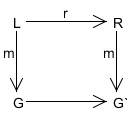
\includegraphics[scale=0.7]{./Figures/GraphTransformationGeneral.png}
    \rule{35em}{0.5pt}
  \caption[Applying model transformations by graph transformations]
  {The basic idea for graph transformation by applying a rule r.}
  \label{fig:categoryTheory}
\end{figure}

For a production rule r, \mbox{G$\xrightarrow{r,m}$G'} indicates a direct
derivation to a derived graph G'. If there is a match m of nodes and arrows for a
subgraph L in a host graph G, then this indicates a graph homomorphism, mapping
elements from the subgraph to the host graph in such a way that the graphical
structure in G is preserved.

\section{The Attributed Graph Grammar System}

\noindent AGG is a general development environment for algebraic graph
transformation systems. AGG is provided with a graphical editor for creating
and modifying graphs. The editor provides a graphical user-interface with
several visual editors for applying the principles of graph transformation. It
also has an interpreter and a set of validation tools. AGG is ongoing research
activity of the graph grammar group at TU Berlin. The work on AGG started back
in the beginning of 1997.

\subsection{Graphical Editor}
\noindent The graphical editor of AGG has several functions to help the user to
define model transformations. In the top left corner of the graphical user-interface is
a tree based editor for defining rules and grammar. This tree based editor also
contains the type graphs and the host graphs. Where the host graph represents
some input model for a model transformation.

\indent Each application rule has two visual editors, representing the left and
the right hand side, or the pattern and the replacement graph. In the tree
based editor containing rules and grammars it is possible to give rules application
conditions. This is convenient if the user wants to have constrains for the
pattern or the replacement graph.

\indent In the tree based visual editor it is also possible to define host
graphs and type graphs. Type graphs is described more in depths in the next
section, but roughly said, the type graph defines elements that can be used in
the host graph. Type graphs defines the abstract models for the host graph and
can be compared to Meta Object Facility (MOF)\cite{MOF}, that is a language for
defining abstract syntax of modeling languages. The users can now create instances
from these type graphs. These instances represents the host graphs and
corresponds to its concurrent type graph. 

\indent For the application rules, the user can extend the attributes with Java
expressions. This means that the users can use Java primitives such as strings,
integers or float numbers to form the pattern graph or the left hand side of
the rule. The user cannot bind attributes that is not initialised in the type graph. 

\begin{figure}[H]
	\centering
	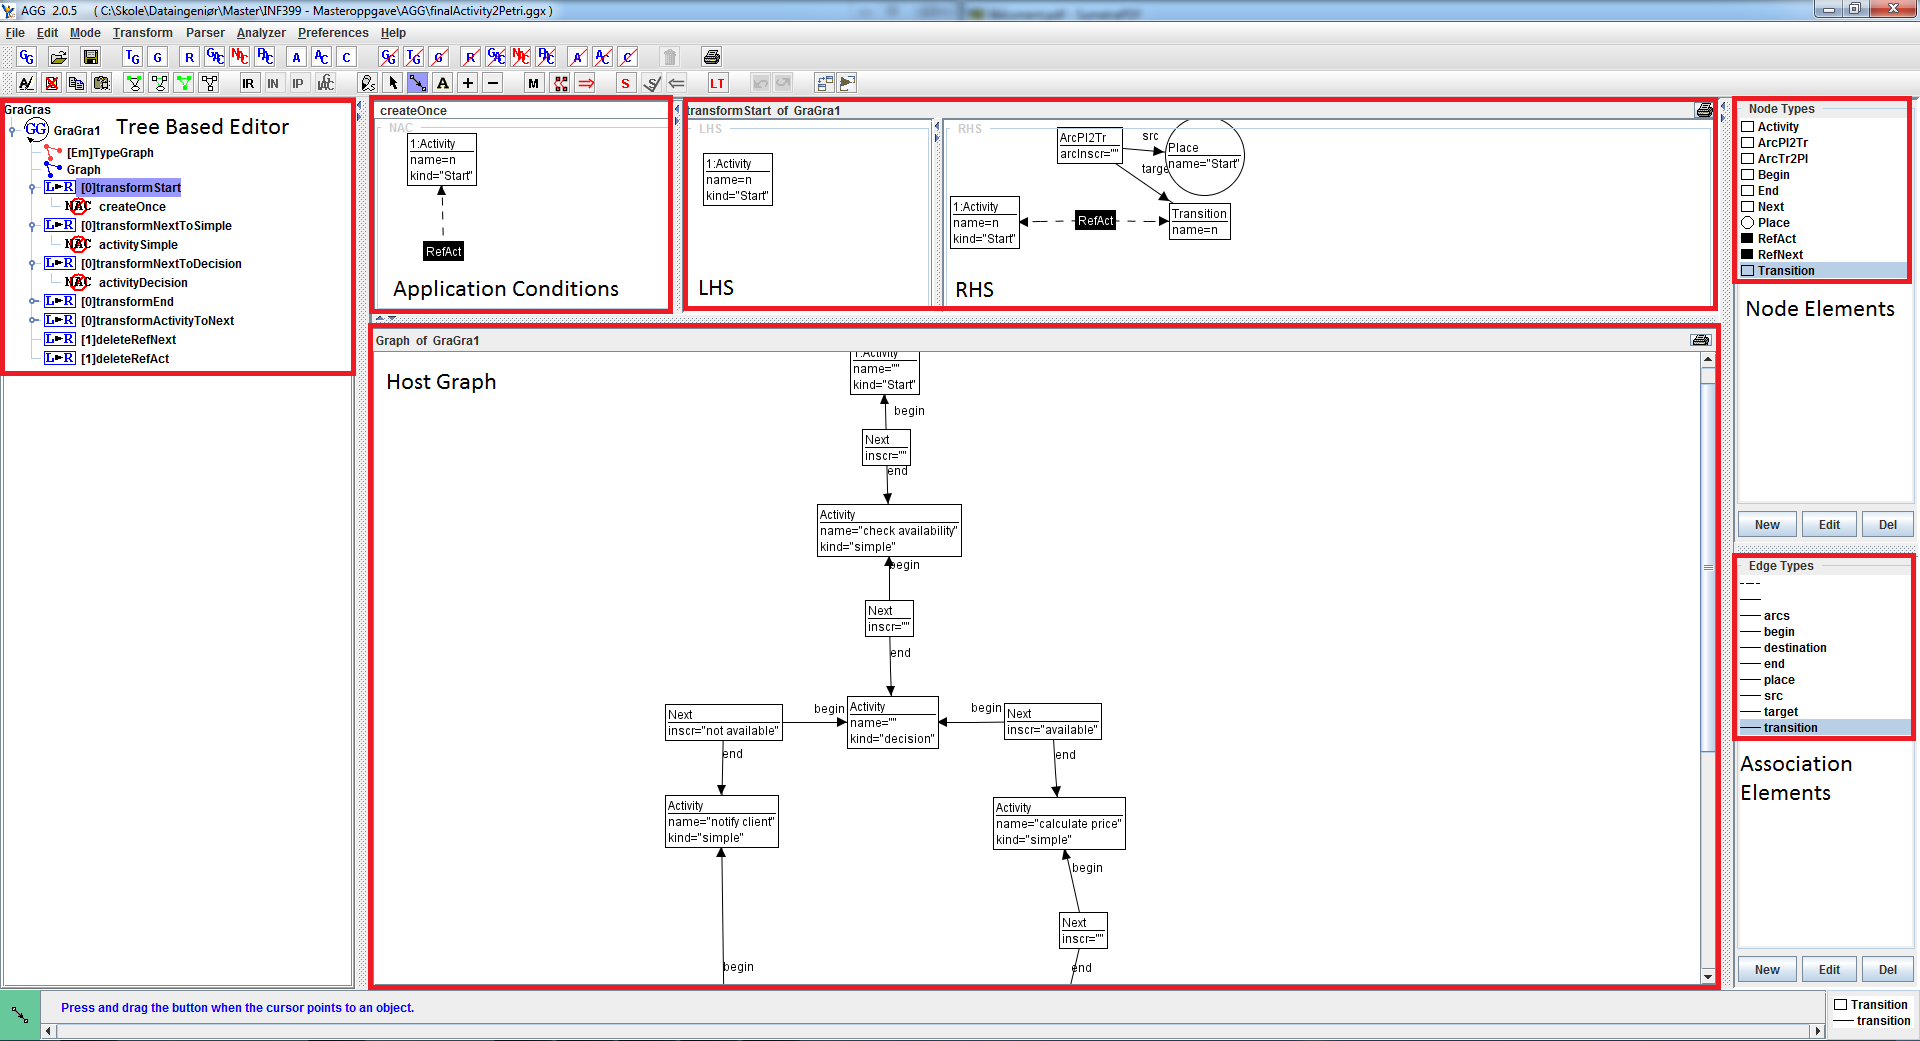
\includegraphics[scale=0.3]{figures/AGGscreen.png}
	\caption{Activity2PetriNets for AGG.}
	\label{fig:AGGScreen}
\end{figure}

\subsection{Type Graph}

\noindent Before the host graphs can be created. a type graph has to be
initialised. These type graphs represents the abstract syntax for the host
graphs. For this case study we created a type graph enabling translation from
an activity diagram to petri nets. Unlike Henshin, the AGG graphs does not
allow for separately definitions of type graphs. Henshin allows the use of one
source and one target metamodel independent of each other. If we want to
prepare an AGG graph for a transformation, we create a single type graph with
references between elements of both source and target metamodel. This way, when
the application rules is executed, we can choose to keep both the source graph
and the references between these elements. The references and source graph can
be deleted through a cycle of transformation rules.

\begin{figure}[H]
	\centering
	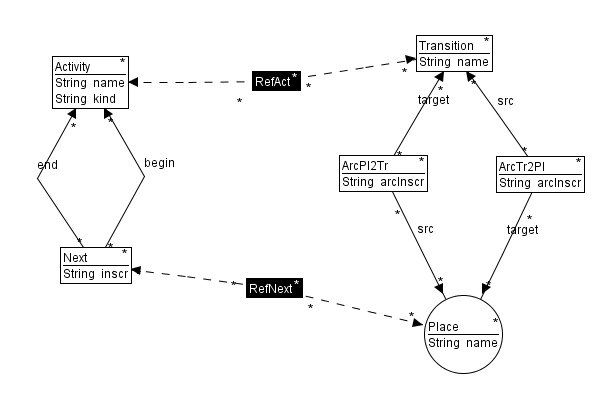
\includegraphics[scale=0.7]{figures/AggTypeGraph.png}
	\caption{Activity diagram to petri nets type graph in AGG.}
	\label{fig:AggTypeGraph}
\end{figure}

\indent For the type graph, the user must define nodes and arrows for each meta
element for both source and target model. These nodes and arrows can also have
attributes. Nodes represents elements from the two modelling languages and
arrows represents the associations between these elements. In the type graph we
want to distinguish between associations and references, and therefore we
represent references as a dashed edge. These dashed edges are not given any
attributes, and that is because we want these edges to represent what the
targeted element was translated from. From figure~\ref{fig:AggTypeGraph} we can
see that a RefAct node is defined and is connected between the activity
element and the transition element. The same initialisation is defined between
the next element and the place element. For AGG type graphs there is a
multiplier condition for the edges. This means that there can be an arbitrary,
or a zero to many number of instances of these relations in the host graph.

\section{The Henshin Project}

\noindent The Henshin project\cite{Henshin} provides a model transformation
language for the Eclipse Modelling Framework \cite{Steinberg2009}. With support
for both direct transformation of EMF single model instances, and translation
from source model to targeted model. The Henshin project is a transformation
language with a provided graphical syntax. With the help of this graphical
editor, it provides the user with an intuitive way of representing rules. 

\subsection{Graphical Editor}
\noindent Henshin model transformation language is a plugin for the Eclipse
Integrated Development Environment\cite{Eclipse}. The Henshin project provides
the users with a graphical editor to create and modify model to model
transformations. 

The users start out with using the Eclipse wizard to create an empty Henshin
document. The henshin document is based on the commonly known Extensible Markup
Language (XML)\cite{XML}. If applicable a Henshin diagram file can be created
based on the Henshin file. This gives the users an intuitive approach to
creating model transformation rules.

The Henshin transformation file is represented in a tree based editor in
Eclipse. In this tree based editor it is possible to include metamodels for both
the source and the target model. These metamodels are created based on the EMF
standard for creating models, that we talked about in the first chapter.
This approach differ from the AGG approach we saw in section 3, where we have
to create both target and source metamodel in one common type graph. In Henshin
the two metamodels are independent of one and another, therefore they are
included as two separate models in the Henshin file. 

\begin{figure}[H]
	\centering
	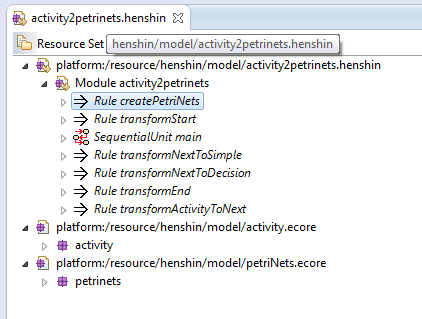
\includegraphics[scale=0.7]{figures/Henshin_TreeEdtiro.png}
	\caption{Tree Based Editor for rules in Henshin.}
	\label{fig:Henshin_TreeEditor}
\end{figure}

\subsection{Defining transformation rules}

\noindent In Henshin, objects are referred to as nodes and links between objects
as edges. A collection of these nodes and edges form a graph. For each graph, a
rule has to be defined. These rules can have parameters for checking and model
verification. Each rule can be represented as a graph in the graphical
editor. 

\indent When creating these rules, there has to be a way of
distinguishing elements between the LHS and the RHS. This is done through the
use of a set of predefined tag words, or stereotypes. For handling transformations
either in the pattern graph or the replacement graph, we can use the three
predefined words <<preserve>>, <<create>> or <<delete>>. <<forbid>> and
<<require>> are used for defining Negative Application Conditions (NACs) and
Positive Application Conditions (PACs). These actions are supported for nodes,
edges and attributes. 

\begin{figure}[H]
	\centering
	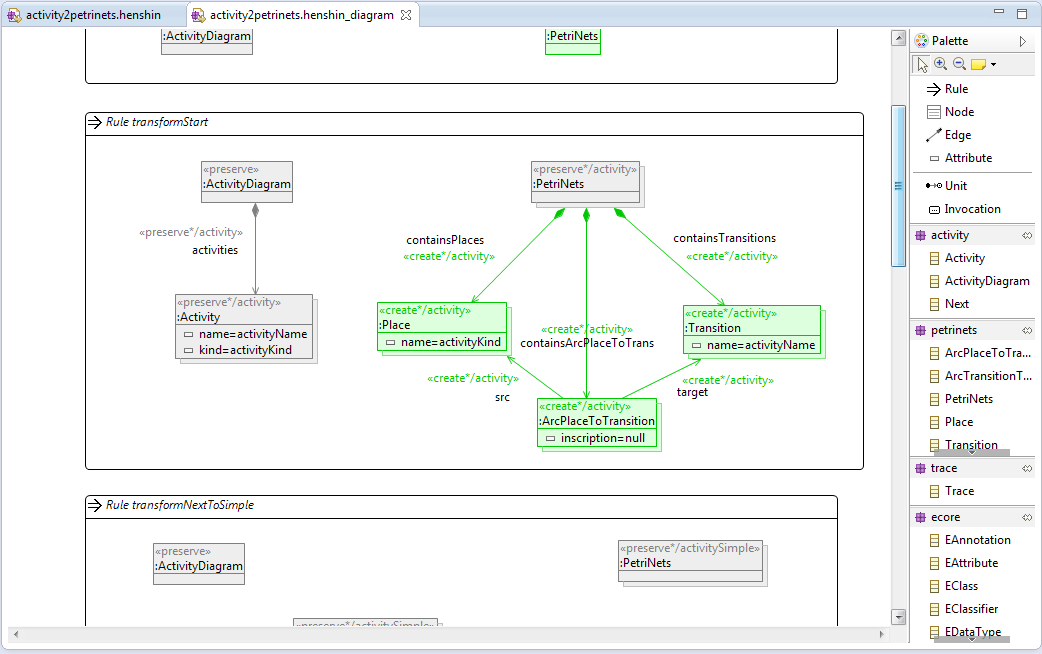
\includegraphics[scale=0.5]{figures/HenshinScreen.png}
	\caption{Activity2PetriNets for Henshin}
	\label{fig:HenshinScreen}
\end{figure}

\section{ATL Transformation Language}

\noindent ATL\cite{ATL} (ATL Transformation Language) is a model transformation
language and is defined as a direct answer to the QVT\cite{QVT} standard. It
provides ways to produce a set of target models from a set of source models.
ATL is developed on top of the Eclipse platform and is one of three
transformation engines provided by the MMT project\cite{MMT}. MMT is a sub
project of the top level Eclipse Modeling Project\cite{EMP}.

\subsection{Syntax based editor}

\noindent ATL can be looked upon as a programming language, because it is
basically a transformation language. ATL is a syntax based transformation
language, and is build around the Object Constrain Language (OCL) \cite{OCL}
with some additional predefined functions. ATL transformations is stored in a
file extension called ``.atl'' These ATL files can contain different kind of
ATL units and are defined in its own distinct ATL file. These different ATL
units are ATL modules, ATL queries and ATL libraries. Libraries can be used to
create independent ATL libraries that can be imported to different types of ATL
units. The module unit specifies the different application rules for a model to
model transformation. And the Queries are used when the users want to compute
primitive values from the source models.

Now that we have specified these three ATL units, we can describe shortly how
we can use the ATL transformation language to create model to model
transformations. For our test case, we only need the ATL modules. An ATL module
corresponds to a model to model transformation. This unit enables developers to
specify the way to produce a set of target models from a set of source models.
The source and target models of an ATL module must be consistent with their
respective metamodels. 

At first, the user start out with a blank ATL file. Since we are working in
the ATL Integrated Development Environment for Eclipse, we want to start the
document with defining the path to the source and target metamodel. The
reason for doing this is to achieve auto completion from the ecore metamodels.
This is convenient for the users when creating transformation rules. 

\begin{figure}[H]
	\centering
	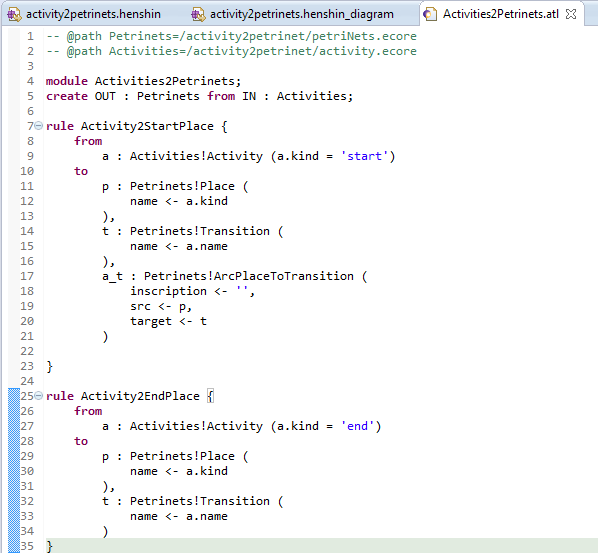
\includegraphics[scale=0.5]{figures/ATLScreen.png}
	\caption{Two simple rules for Activity2PetriNets in ATL.}
	\label{fig:ATL_Screen}
\end{figure}

Next the
file is composed of four different elements. The first element is the header
section, where the user can give the module a name and name the variables
corresponding from the source and target models. The module name has to be
identical to the name of the ATL file. We also need to specify a way to
distinguish between source and target models. The target models declaration is
introduced with the keyword create, and the source models are introduced using
the keyword from. The user can also import some existing libraries if needed.
This import section is however optional. The third element in a ATL module is a
set of helpers. This collection of helpers can be compared to Java methods.
These helper methods can be used to make the transformation rules easier to read
for example. The last element is a set of rules that defines how the target
models are generated from the source models. These rules are used to implicitly
match source elements and produce target elements. 

\subsection{Principles behind execution}

\begin{figure}[H]
	\centering
	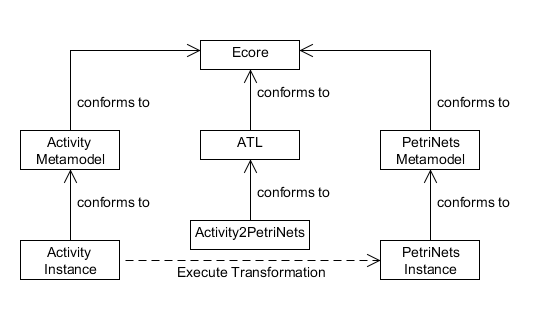
\includegraphics[scale=0.5]{figures/ATL.png}
	\caption{Model transformation process for Activity2PetriNets.}
	\label{fig:ATL}
\end{figure}

This diagram gives us an idea of how the ATL transformation from an activity
diagram to petri nets are handled. We want to generate a model PetriNets
instance, that conforms to the metamodel PetriNets. This is generated from a
source model, Activity Instance, that conforms to its respective metamodel.
The created transformation Activity2PetriNets is expressed in the ATL
transformation  language, that conforms to its own metamodel. These three
metamodels conform to the metamodel Ecore. So this makes Ecore a metametamodel
for the other three metamodels. 

\section{Evaluation}
\noindent Now that we have worked with these tools, we have to evaluate them.
From the table underneath we have tried to compare the different tools, and we
will explain some of them in further detail. We should start talking about how
easy or hard these tools were to learn. It took some time to fully understand
how graph transformations work. That there are a right hand and a left hand
side of each rule, and that these rules also can have both negative and
positive application conditions. But after a while, when the aspects around
graph transformation got clearer, the tools were easier to handle. AGG was the
first tool i encountered, my learning curve became steep after i learned how
graph transformations works. AGG has a clear procedure on how to create and
manage new application rules. AGG is also very intuitive to work with, as long
as the users understands how graph transformation steps works. After spending
time on AGG and its graphical editor to create transformation rules, the next
stop was Henshin. My learning curve for Henshin was not as steep as AGG, but
this tool was also very nice once the knowledge of it was present. After
tackling the problems that Henshin brought along it was time to look at the
ATLAS Transformation Language. And this tool is a very nice tool to write model
to model transformation. Its definitely not as intuitive as the two graph
transformation tools, but that is common issue when learning a new tool, no
matter what it is used for. Once you understand how to create transformation
rules and how to work with the included metamodels it is a nice framework for
working with model transformations. However, if a user do not fully understand
the Object Constraint Language (OCL), ATL is rather a hard tool to work with.
Because OCL has a very leveled learning curve, since it is a declarative
programming language. Where we are more or less used to work with imperative
programming languages during our studies here in Bergen.

\begin{table}[ht]
\centering
\begin{tabular}{| c | c | c | c |}
\hline
 & AGG & Henshin & ATL \\
\hline
Endogenous transformation & \cellcolor{green!25}Yes &
\cellcolor{green!25}Yes & \cellcolor{green!25}Yes \\

Exogenous transformation & \cellcolor{green!25}Yes &
\cellcolor{green!25}Yes & \cellcolor{green!25}Yes \\

Input Elements & 1\ldots n & 1\ldots n & 1\ldots n\\
Output Elements & 1\ldots n & 1\ldots n & 1\ldots n\\
Inplace/outplace model transformation &inplace &
inplace &outplace \\
Graphical syntax &\cellcolor{green!25}Yes &
\cellcolor{green!25}Yes &\cellcolor{red!25}No  \\
Integrated with Java & \cellcolor{green!25}Yes &
\cellcolor{green!25}Yes & \cellcolor{green!25}Yes \\
Supports EMF & \cellcolor{red!25}No &
\cellcolor{green!25}Yes & \cellcolor{green!25}Yes \\
Separate metamodels & \cellcolor{red!25}No &
\cellcolor{green!25}Yes & \cellcolor{green!25}Yes \\
\hline

\end{tabular}
\caption{Comparing model transformation tools.}
\end{table}

From the table above, we can see that all the three tools have support for both
endogenous and exogenous model to model transformations. For Henshin and ATL
this means that there is support for both direct transformation of single EMF
model instances and translation from source model instances to a target model
written in another modelling language. One thing that is worth mentioning is
that AGG does not have support for EMF, the transformation engine that comes
with AGG can be integrated with Java, and therefore it can be supported with
EMF, but this has to be integrated manually. This is a very nice feature for
Henshin and ATL, that they support the popular modelling framework EMF. This
means that the users can create metamodels in the Ecore modeling language and
use these metamodels in Henshin or ATL. 

All the three tools has support for an arbitrary number of both input and output
elements. The ATL module accepts a fixed number of models as input, and returns
a fixed number of target models. This means that an ATL module can not generate
an unknown number of target models. If there is one input model, then there
will be one output model that conforms to a given metamodel.

Both AGG and Henshin have a graphical editor, where the users can type in
graphical syntax to create transformation rules. This makes them both very
intuitive for the users. This is not the case for ATL, where this tools uses a
syntax based approach. This means that the users have to implement
transformation rules. This is a very nice approach if the users master the mix
between the ATL transformation language and the OCL programming language.

When ATL transformation language executes the application rules for the model to
model transformation, a new model instance is created for the target model. This
means that the source model and the target model are independent of eachother.
Where Henshin and AGG performs in-place model to model transformations. This
means that they both operate on the host graph, and translates the models inside
the host graph. All three approaches can however give the same result. Inn AGG
and Henshin the users just need to make sure to delete unwanted elements from the
translated host graph. On the other side, for ATL this is not needed, since both
the source and target model are kept as separated files. 

All three tools can be integrated with Java. The problem with ATL is that there
has to be a ``atl'' file containing the ATL module. This is because the ATL
transformation engine relies on a file extension with the name ``atl''. The
graphical editor that AGG provides runs on top of a separate transformation
engine. AGG's transformation engine can take java objects as input parameter and
manipulate models from these java objects.

And lastly we can sum up how these tools handles the source and target
metamodels. Henshin and ATL includes them pretty much the same way. They have
one seperate source metamodel and one seperate target metamodel. In ATL the
users has to explicitly assign the metamodels to either source model or target
models through the ATL run configuration. The run configuration is when the
model to model transformation is initiated. So this needs to be configured with
assigning the appropriate metamodel to the appropriate models. Henshin on the
other hand includes the metamodels in the henshin model transformation file. Now
it is up to the users who model these transformation rules to make sure that the
models are consistent with their respective metamodels. This is done when
carefully assigning the source and target model to either the right hand side or
the left hand side of the transformation rule. AGG on the other hand uses a
disjoint metamodel. This means that in AGG there is something called a type
graph, and in this type graph both the target and the source metamodel are
defined. From figure \ref{fig:AggTypeGraph} in chapter 3, we can see that there
are created references between these two metamodels. And through the use of
these references, AGG can create and modify application rules to translate
amongst two models.

%-----------------------------------
%	SUBSECTION 1
%-----------------------------------
\subsection{Subsection 1}

Nunc posuere quam at lectus tristique eu ultrices augue venenatis. Vestibulum ante ipsum primis in faucibus orci luctus et ultrices posuere cubilia Curae; Aliquam erat volutpat. Vivamus sodales tortor eget quam adipiscing in vulputate ante ullamcorper. Sed eros ante, lacinia et sollicitudin et, aliquam sit amet augue. In hac habitasse platea dictumst.

%-----------------------------------
%	SUBSECTION 2
%-----------------------------------

\subsection{Subsection 2}
Morbi rutrum odio eget arcu adipiscing sodales. Aenean et purus a est pulvinar pellentesque. Cras in elit neque, quis varius elit. Phasellus fringilla, nibh eu tempus venenatis, dolor elit posuere quam, quis adipiscing urna leo nec orci. Sed nec nulla auctor odio aliquet consequat. Ut nec nulla in ante ullamcorper aliquam at sed dolor. Phasellus fermentum magna in augue gravida cursus. Cras sed pretium lorem. Pellentesque eget ornare odio. Proin accumsan, massa viverra cursus pharetra, ipsum nisi lobortis velit, a malesuada dolor lorem eu neque.

%----------------------------------------------------------------------------------------
%	SECTION 2
%----------------------------------------------------------------------------------------

\section{Main Section 2}

Sed ullamcorper quam eu nisl interdum at interdum enim egestas. Aliquam placerat justo sed lectus lobortis ut porta nisl porttitor. Vestibulum mi dolor, lacinia molestie gravida at, tempus vitae ligula. Donec eget quam sapien, in viverra eros. Donec pellentesque justo a massa fringilla non vestibulum metus vestibulum. Vestibulum in orci quis felis tempor lacinia. Vivamus ornare ultrices facilisis. Ut hendrerit volutpat vulputate. Morbi condimentum venenatis augue, id porta ipsum vulputate in. Curabitur luctus tempus justo. Vestibulum risus lectus, adipiscing nec condimentum quis, condimentum nec nisl. Aliquam dictum sagittis velit sed iaculis. Morbi tristique augue sit amet nulla pulvinar id facilisis ligula mollis. Nam elit libero, tincidunt ut aliquam at, molestie in quam. Aenean rhoncus vehicula hendrerit.